\documentclass[12pt]{article}

% Packages
\usepackage[T1]{fontenc}
\usepackage[margin=1in]{geometry}
\usepackage{amsmath,amssymb}
\usepackage[numbers,sort&compress]{natbib}
\usepackage{graphicx}
\usepackage{booktabs}
\usepackage{xcolor}
\usepackage{hyperref}
\graphicspath{{../../../figures/}}

\title{Sea level is likely to rise more than 1 meter in the 21st century}
\author{Minchew, Meyer, et al.}
\date{}

\begin{document}
\maketitle

%% ================================================================
\begin{abstract}

Every centimeter of sea-level rise exposes roughly 1.6 million additional people to coastal flooding, yet the projections guiding adaptation planning rely on models that diverge below observed trends within a decade. We construct a data-driven sea-level forecast by calibrating reduced physical models for individual sea-level contributors against decades-long independent observational records. When forced with observed surface temperatures, the calibrated components sum to match observed global mean sea level rise (GMSLR) within error. Our forecasts show a 73\% probability of GMSLR exceeding 1 meter, and 10\% of exceeding 2 meters, by the end of the century. The dynamics of West Antarctic glaciers account for $>90$\% of the forecast uncertainty and reveal orthogonal dimensions of sea-level risk: emissions reduction decreases contributions from the predictable, temperature-sensitive components, but leaves the high-risk tail of the distribution largely unchanged, exposing hundreds of millions of people to accelerating flood risks.

\end{abstract}

%% ================================================================

Rates of global mean sea-level rise (GMSLR) have doubled twice in the past 50 years \citep{Frederikse2020,Hamlington2024} (Fig.~\ref{fig:observations}). The first doubling took about 16 years and $0.34\ ^\circ$C of warming \citep{Rohde2020}. The second took about 21 years and $0.41\ ^\circ$C of warming (Fig.~\ref{fig:observations}). The rate could double again around 2080 if the current observed sea-level acceleration continues, and by 2040 if it takes no more warming than the previous two doublings. The 40-year gap illustrates the uncertainty that coastal planning and adaptation must absorb.

%% ---- Figure 1: Observations ----
\begin{figure}[t]
\centering
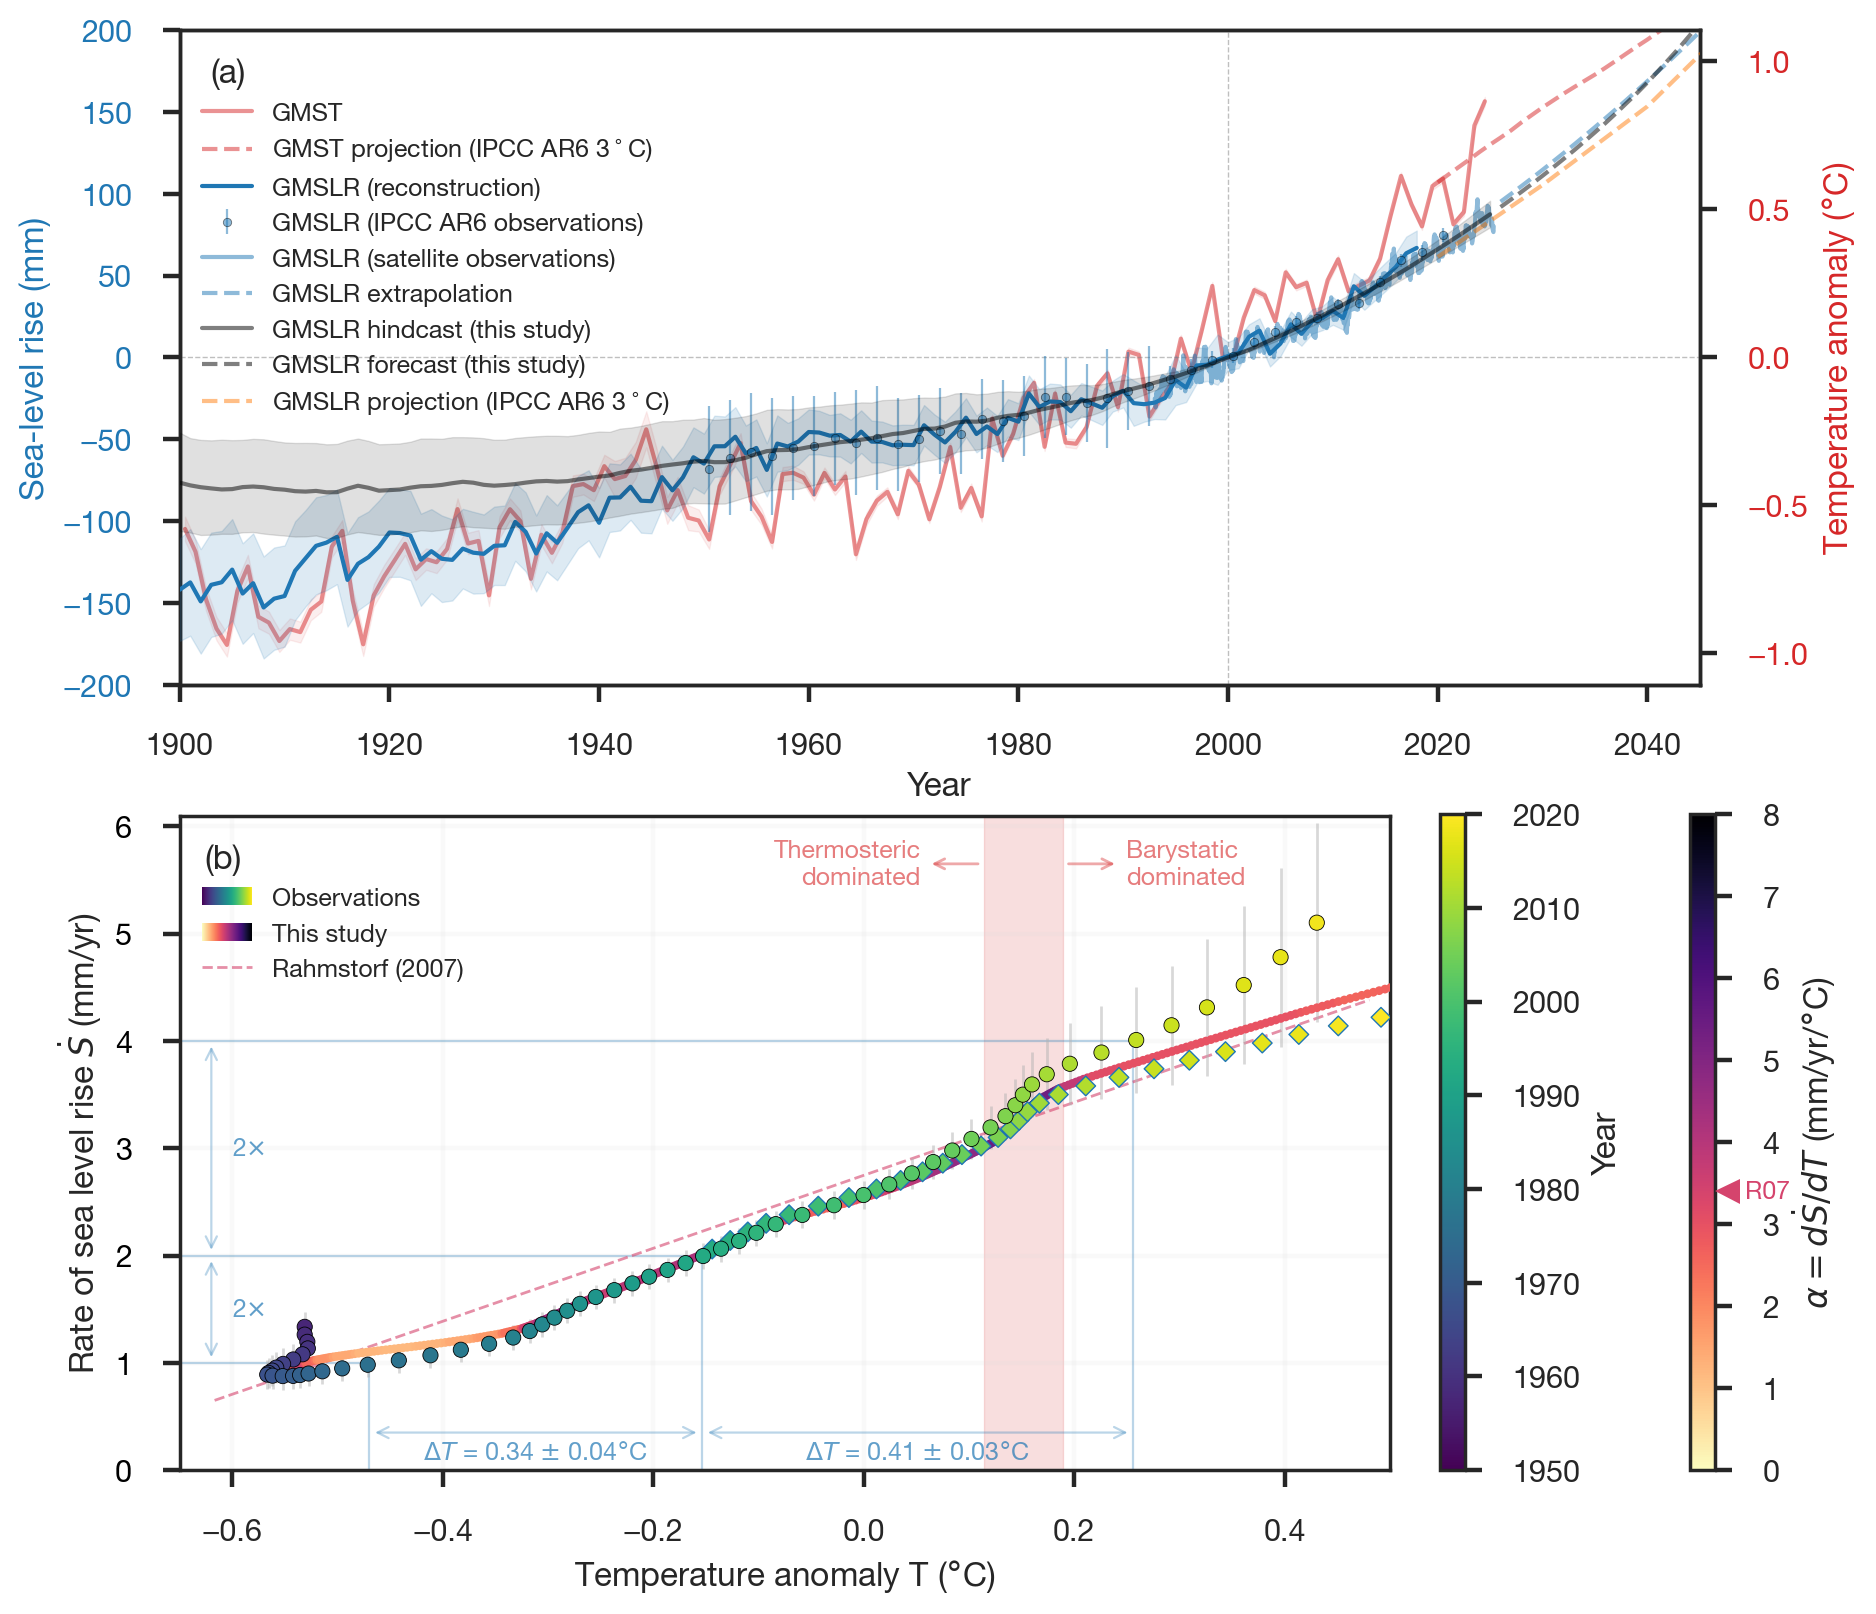
\includegraphics[width=\textwidth]{fig1v2_observations.png}
\caption{\textbf{Observed global mean sea-level rise and its response to global mean surface temperature.}
\textbf{(a)}~GMSLR (blue, 5-year smooth; \cite{Frederikse2020}) and NASA satellite altimetry (light blue; \cite{Beckley2017}), with the satellite-era extrapolation (dashed; \cite{Hamlington2024}). GMST (red, 15-year smooth~\cite{Rohde2020}) is referenced to the righthand axis.
\textbf{(b)}~Rate of GMSLR ($\dot{S}=dGMSLR/dt$) versus GMST anomaly, $T$.  Observed values are shown in circles \cite{Frederikse2020} and diamonds \cite{Beckley2017}, colored by year, and the component model of this study is a line colored by instantaneous transient sensitivity $\alpha = d\dot{S}/dT$. The Rahmstorf (2007) semi-empirical model is shown in a color corresponding to its $\alpha$ value \citep{Rahmstorf2007}. The vertical red band indicates the shift in the primary contributor from ocean thermal expansion changes in glacier ice and water storage (barystatic). The sinuous tail in the early observations is largely due to dam impoundment of water rather than a thermodynamic signal~\citep{Frederikse2020}. }
\label{fig:observations}
\end{figure}

Every centimeter of sea-level rise exposes roughly 1.6 million additional people to annual coastal flooding \citep{Kulp2019}, approximately 90\% of whom live in low- and middle-income countries \citep{Jongman2012}. Without additional adaptation, annual flood damages are projected to reach US\$14--18~trillion per year for 0.9--1.1~m of rise \citep{Jevrejeva2018}. Estimates of total adaptation costs per unit sea level rise are not available but a lower-bound, rough-order-of-magnitude estimate of US\$4~trillion per meter of sea-level rise is reasonable based on a projected cost of US\$400~billion simply to raise dikes by 1 meter along only 3.4\% of coastlines \citep{Tiggeloven2020}. Developing countries currently receive US\$21~billion per year in total adaptation finance across all sectors, not just coastal \citep{UNEP2023}, raising serious questions about the feasibility of coastal adaptation at relevant scales and highlighting the extreme financial costs, to say nothing of human and ecological impacts, arising from large uncertainties.

The rate of reduction in the uncertainties is a crucial consideration because effective planning requires reliable sea-level forecasts be delivered before key decisions need to be made. Uncertainty in the rates of sea-level rise compounds uncertainty in inundation thresholds and paralyzes anticipatory spatial planning, routinely defaulting policy toward \emph{in situ} maladaptations that compound sunk costs and strand assets \citep{ODonnell2022}, or delaying action until forced by disaster \citep{Tubridy2021}. Unconstrained timelines encourage fragmented, market-based incrementalism that deploys public capital inefficiently \citep{SidersAjibadeCasagrande2021} and systemically transfers the financial burden of reactive retreat onto vulnerable municipalities and demographics \citep{SidersAjibade2021}. 

Current coastal adaptation planning relies heavily on projections from the IPCC Sixth Assessment Report (AR6), which estimates 0.4--0.7~m of rise by 2100 relative to the 1995--2014 baseline \citep{Fox-Kemper2021, Hirschfeld2023}. These projections depend largely on process-based ice sheet models that diverge from satellite observations within years of initialization \citep{Aschwanden2021, Fricker2025}. As a result, observed GMSL trends (0.66 m median at 2100, 0.41--0.91 m 90\% CI) already exceed AR6 medium-confidence projections under all policy-relevant emission scenarios \citep{Hamlington2022, Hamlington2024}. AR6 itself documents this in a single figure but without comment: extrapolating the satellite-era rate and acceleration---which reflect the current warming trajectory that could lead to $3\ ^\circ$C (SSP2-4.5)---produces sea-level rise that matches or slightly exceeds the process-based projections under the very high emissions scenario (SSP5-8.5), which is now regarded as generating an implausible level of warming (AR6 Figure~9.27; \citep{Fox-Kemper2021,Hausfather2020}). So while the data show that rates of sea level rise double with approximately 0.4~$^\circ$C of warming (Fig.~\ref{fig:observations}b), IPCC models need roughly an order of magnitude more warming just to reproduce current observed rates of sea-level rise. 

Disagreement between observations and ice sheet models arise from known structural biases, including the absence of leading-order physical processes like iceberg calving \citep{Fricker2025} and an assumed ice viscosity that is less sensitive to stress than observations indicate \citep{Millstein2022}. The latter produces a roughly 30\% underestimate of projected 21st century ice loss, exceeding the uncertainty due to warming trajectories \citep{GetraerMorlighem2025}. More broadly, decades of general forecasting research shows that models more complex than their calibration data can constrain produce worse predictions than simpler models \citep{Green2015, Makridakis2020}. Current ice sheet models have millions of degrees of freedom representing spatially distributed parameters and uncertain parameterizations. The observations used to initialize these models inform only a small fraction of these degrees of freedom, with the remainder determined by prior assumptions and model design \citep{Isaac2015, Petra2014}. A forecasting system based on models representing diverse approaches and a hierarchy of complexity is needed to fill the needs of coastal planning for sea-level rise.

\subsection*{Data-driven forecasting}

We construct a data-driven forecast that focuses on different sea-level contributors, each with minimal physical models constrained by independent observational records spanning decades. Observed GMSLR and its sensitivity to observed global mean surface temperature (GMST) are diagnostics, and we show that the sum of our model components agrees within 6\% of 2000--2025 observed GMSL in hindcasting tests (Supplementary Material). Unless otherwise noted, all sea-level values in the main text are global-mean 21st-century contributions referenced to the year 2000, while values in the abstract are relative to pre-industrial for consistency with existing projections and literature. Throughout, we label emission scenarios by their approximate end-of-century global mean surface temperature: 2$\,^\circ$C (SSP1-2.6), 3$\,^\circ$C (SSP2-4.5), and 4$\,^\circ$C (SSP3-7.0).

Our framework builds on two established lines of data-driven forecasting. The simplest is the ``naive" forecast, which requires only a fit to the observed GMSL rate and acceleration. The satellite altimetry record provides GMSLR measurements from 1993--2025 that show a constant acceleration of 0.08~mm\,yr$^{-2}$ (0.02--0.14~mm\,yr$^{-2}$) and rate 4.5~mm\,yr$^{-1}$ (3.5--5.5~mm\,yr$^{-1}$) in 2025 \citep{Hamlington2022, Hamlington2024}. Extrapolating these values to 2100 yields 66~cm (41--91 cm) of 21st-century rise (Fig. \ref{fig:ridge_projections}a). Assuming the naive forecast has predictive skill over about half the calibration window, the extrapolation of the 32-year satellite record provides predictive skill over the next 15-20 years. Beyond that horizon, the naive forecast is less reliable but nevertheless establishes a scenario-independent, data-driven reference (Fig. \ref{fig:ridge_projections}a). 

At the next level of complexity are the semi-empirical models that are based on the observed sensitivity of the rate of GMSLR to changes in GMST (Fig.~\ref{fig:observations}b). Under current warming trends, Rahmstorf (2007) \citep{Rahmstorf2007} predicts 0.67~m (0.63--0.71 m) of 21st-century rise, matching the extrapolation of modern observed rates within error \citep{Hamlington2024}. Although physically motivated by the fit to observed sensitivities, semi-empirical models were assessed as \emph{low confidence} by IPCC AR5 because they do not resolve individual contributing processes and because extrapolation beyond the calibration period assumes a stationary temperature--sea-level relationship \citep{Church2013}. This reasoning is carried forward by AR6 but violated by the decision to favor process models that omit key physical processes, are calibrated on non-stationary data, and were not tested against observed GMSL, the very quantity they claim to predict, prior to publication \citep{Fox-Kemper2021}. Our own results show that the simplest semi-empirical models have much greater forecasting skill for the components of sea-level rise that are directly sensitive to warming.  

%% ================================================================
\subsection*{Component forecast model}

We decompose global mean sea level into separate components: ocean thermal expansion (thermosteric), Greenland Ice Sheet (GrIS) surface mass balance (SMB) and glacier discharge, West Antarctic Ice Sheet (WAIS) glacier discharge, East Antarctic Ice Sheet (EAIS) SMB, Antarctic Peninsula total ice loss, glaciers (land ice not in the ice sheets), and terrestrial water storage. Our component-summation approach builds on the methodology of previous studies \citep{Kopp2014,Mengel2016,Wong2017}, while extending to more recent data, initializing the forecasts by blending the calibrated sensitivities with extrapolated observational trends to ensure near-term alignment between the forecast and observed data trends (Supplementary Materials), and developing a structured deep-uncertainty treatment of WAIS discharge. The sensitivities of glaciers, GrIS discharge, and Antarctic Peninsula to warming are calibrated with independent observational datasets spanning 24--71 years (Table~S1). Surface mass balance for GrIS and EAIS are adopted from published model sensitivities rather than data calibration because they lack sufficient data coverage for our approach \citep{Fettweis2020, Noel2021}. For completeness, we adopt the IPCC projection of terrestrial water storage due to a lack of suitable data to support our approach. Details of our models for EAIS and Antarctic Peninsula can be found in Supplementary Materials; we omit them from the main text because their contributions are small enough to be within the uncertainties the primary contributors. 

%% ---- Figure 2: Model calibration, validation, and WAIS uncertainty ----
\begin{figure}[t]
\centering
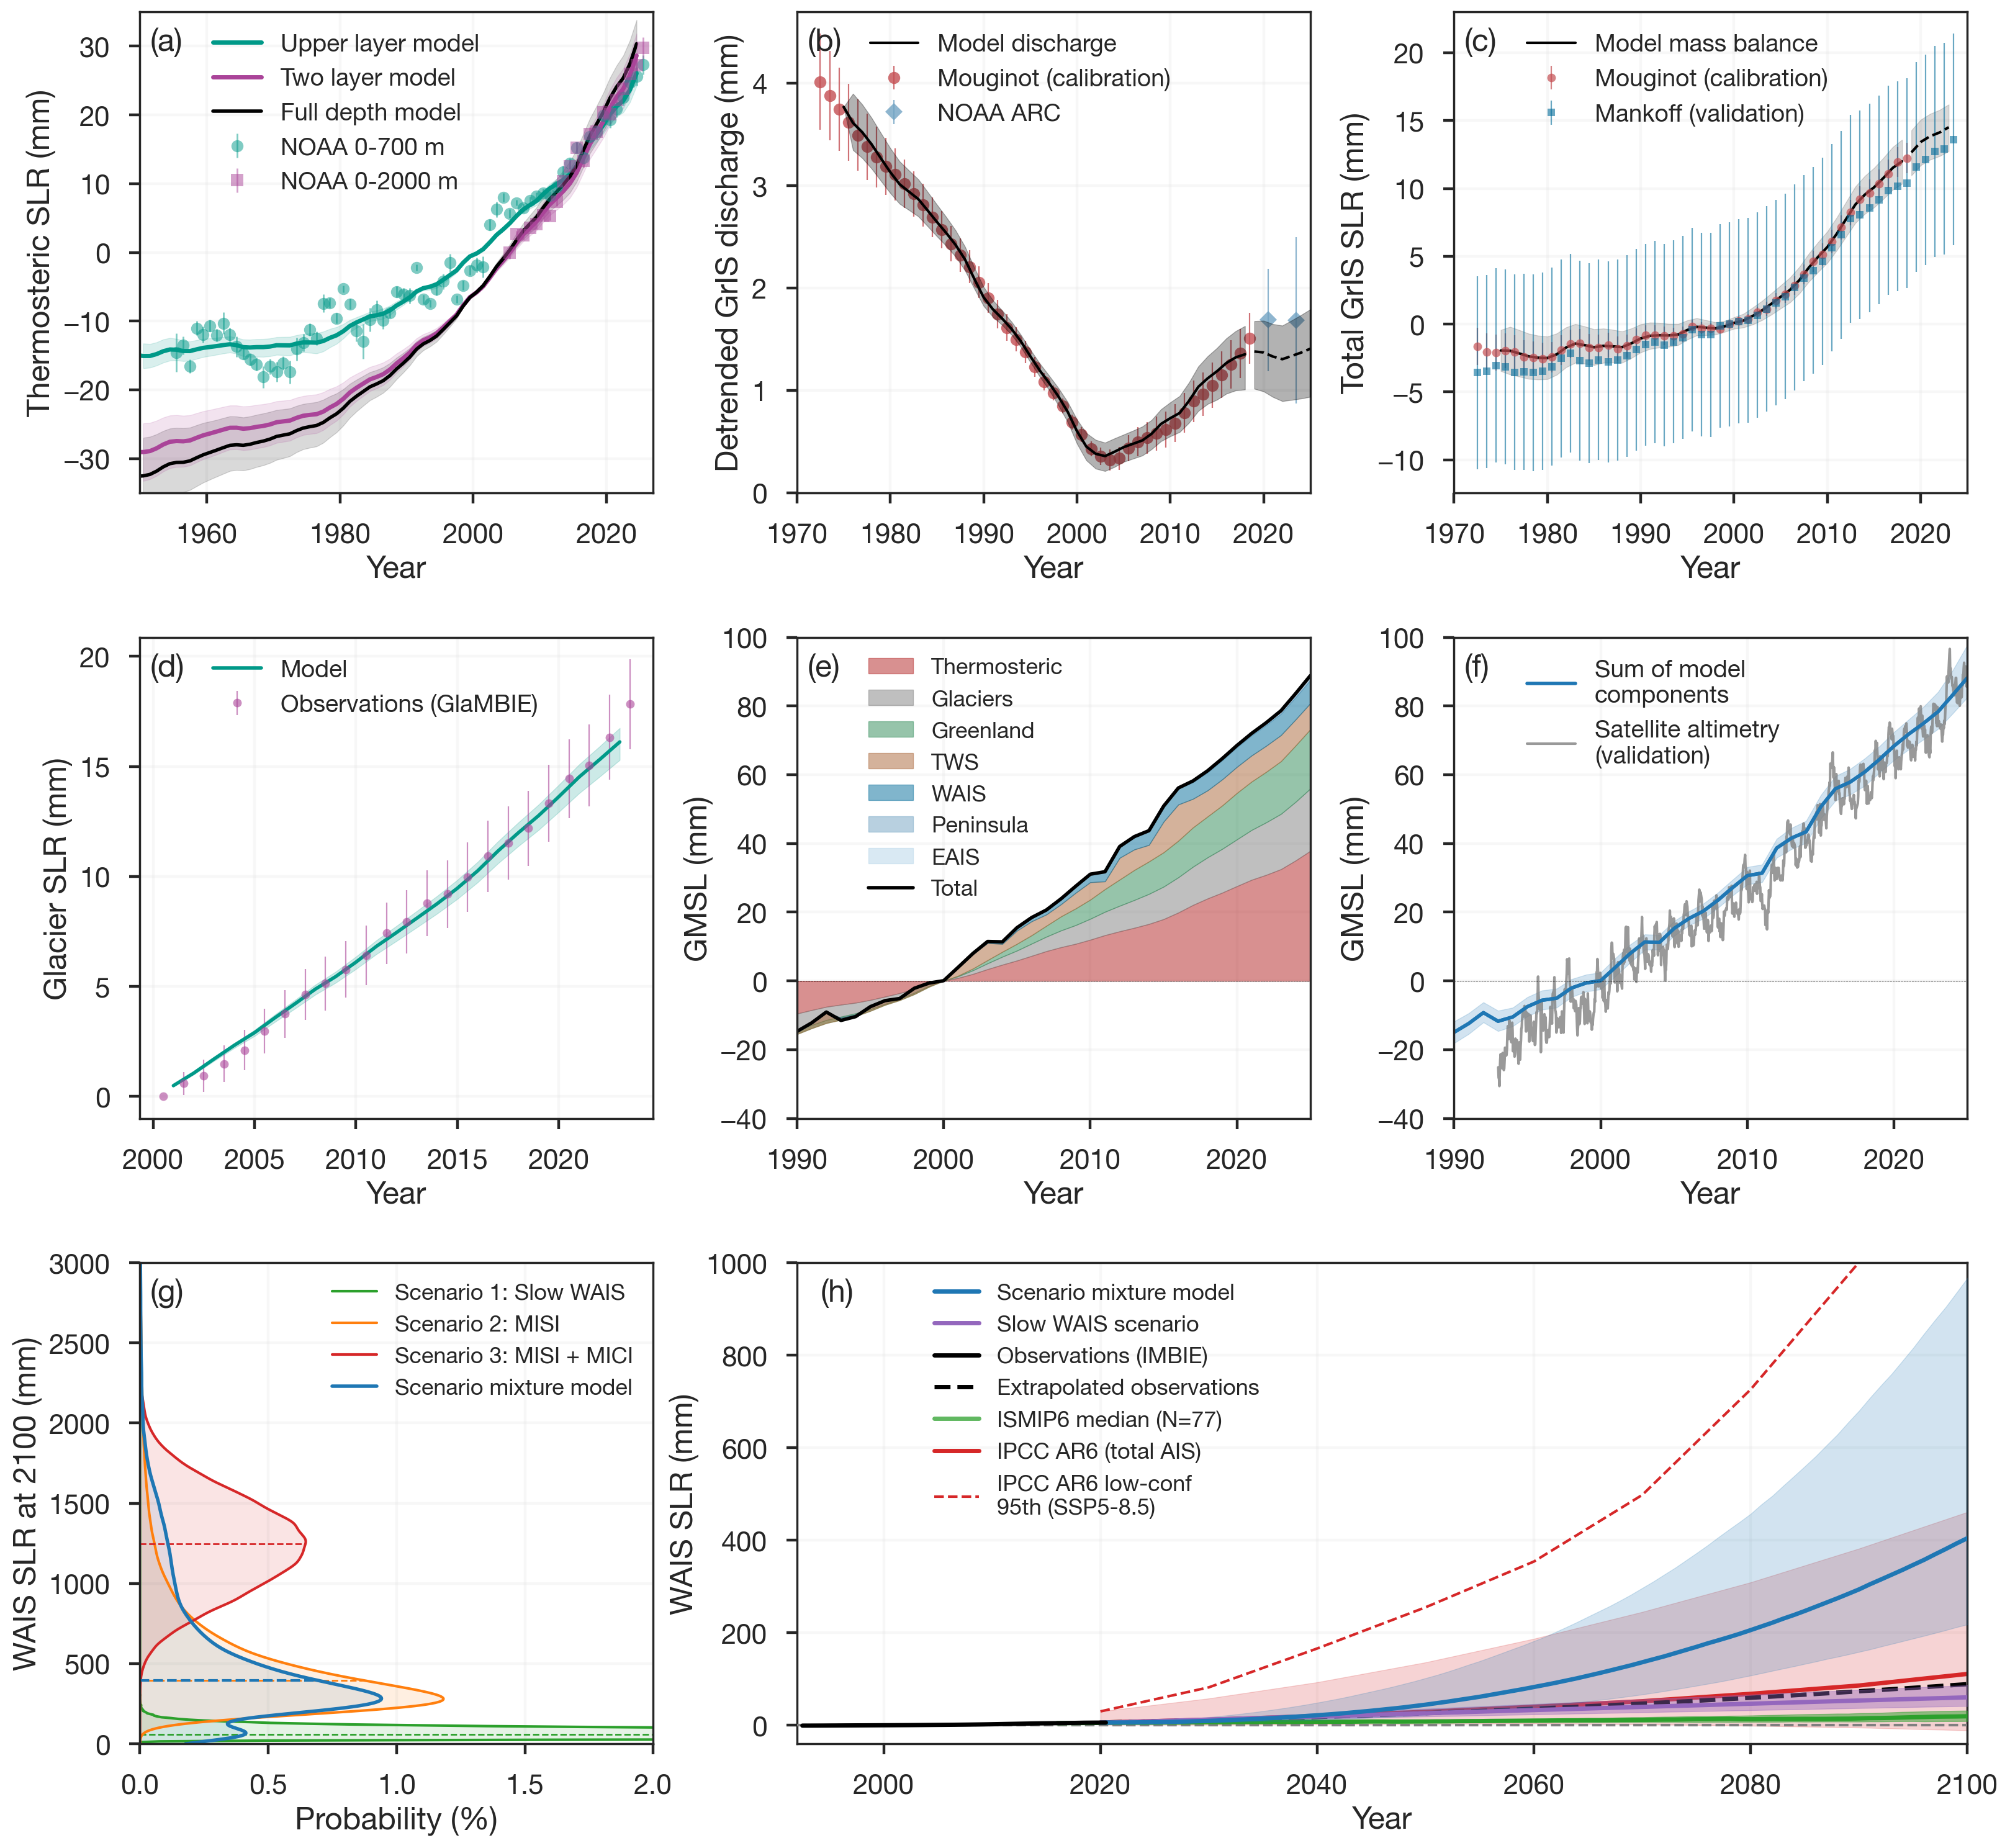
\includegraphics[width=\textwidth]{fig3_calibration_validation.png}
\caption{\textbf{Model calibration, validation, and WAIS uncertainty.}
\textbf{(a)} Our two-layer energy balance model fitted jointly to NOAA thermosteric values at different depth layers with the full depth model used in the forecasts (Supplementary Materials). 
\textbf{(b)} Greenland ice discharge modeled as a cumulative time-delay response to subsurface ocean warming with the calibration data from \citep{Mouginot2019} shown with filled circles and diamonds showing NOAA Arctic Report Card estimates \citep{Poinar2026}.
\textbf{(c)} Greenland total mass balance with validation data shown in blue squares with 90\% CI error bars \citep{Mankoff2021}.
\textbf{(d)} Global glacier model fitted to GlaMBIE consensus observations (2000--2023) using a linear temperature-driven model.
\textbf{(e, f)} Budget closure: temperature-forced component hindcast (stacked) compared with satellite altimetry data.
\textbf{(g)} WAIS scenario distributions at year 2100. 
\textbf{(h)}WAIS projections from our full scenario mixture (blue) and slow WAIS scenario (purple) compared with  observations (black, \citep{Otosaka2023}), the ISMIP6 ensemble (green; \cite{Seroussi2020}), and IPCC AR6 projections (red). }
\label{fig:calibration}
\end{figure}

The thermosteric component is the largest single contributor to observed sea-level rise. We model it with a two-layer energy balance \citep{Geoffroy2013} fitted jointly to NOAA \emph{in situ} thermosteric measurements at 0--700\,m (1957--2025) and 0--2000\,m (2005--2025) \citep{Levitus2012} (Fig. \ref{fig:calibration}a). In our model, the upper ocean responds to GMST warming through a thermal state variable $S_u$ with relaxation time $\tau_u$. The deep ocean thermal state relaxes toward $S_u$ on a longer timescale $\tau_d = 150$\,yr \citep{Geoffroy2013}. We fit the model parameters to the data using a Monte Carlo approach described in Supplementary Material. Forecasts are generated by driving the calibrated two-layer model with IPCC AR6 temperature trajectories, propagating posterior parameter uncertainty via Monte Carlo sampling (Supplementary Material).

The Greenland Ice Sheet is currently the largest land-ice contributor. Its contribution is from imbalances between mass gained through snow accumulation and mass loss from melting and glacier ice discharge. We treat SMB and ice discharge separately. We found that available data are insufficient to constrain SMB, and instead we use regional climate models. For the hindcast, we use RACMO-derived SMB observations \citep{Mouginot2019, Noel2018} directly. For projections, we adopt published linear and quadratic sensitivities of SMB to GMST from RCM intercomparisons \citep{Fettweis2020, Noel2021}, using the spread across RCMs (MAR, RACMO, HIRHAM) as structural uncertainty \citep{Glaude2024} (Supplemental Materials). 

GrIS discharge acceleration is sensitive to ocean temperature \citep{Straneo2013}, and therefore we model it as the cumulative response to time-delayed subsurface ocean warming, with a sensitivity $\gamma$, a delay $\delta$ between ocean warming and glacier response, and a secular drift $r_0$ (Supplementary Material). Using 47 years of glacier discharge data \citep{Mouginot2019} and EN4 ocean temperatures \citep{Good2013}, we find $\delta = 5$~yr, consistent with fjord overturning and glacier dynamics, with sensitivity $\gamma = 0.37$ mm\,yr$^{-1}\,^\circ$C$^{-1}$, which is consistent with scaling estimates from ocean and glacier dynamics (Fig. \ref{fig:calibration}b; Supplemental Material). An independently derived discharge record (1986--2023) \citep{Mankoff2021} and NOAA Arctic Report Card estimates \citep{Poinar2026}, both withheld from calibration, shows our model within 90\% CI, as does the total Greenland mass balance (Fig. \ref{fig:calibration}c), suggesting that our simple 3-parameter model captures the salient physical processes of the observational record. To project this model forward in time, we calibrate a transfer function between the Greenland regional surface temperature anomaly and the ocean temperature and then apply a normal distribution of Arctic amplification factors to calculate the Greenland regional surface temperature form projected GMST under different emission scenarios (Supplemental Material). 

Mountain glacier mass loss is modeled as a rate--temperature relation calibrated against the GlaMBIE global consensus \citep[2000--2023;][]{GlaMBIE2025} and GMST. The data only support a linear sensitivity (Supplementary Material), which we find to be $b_{\mathrm{gl}} = 0.66$~mm\,yr$^{-1}$\,$^\circ$C$^{-1}$ (Fig. \ref{fig:calibration}d). This is approximately five times the value embedded in IPCC AR6 median projections ($\sim$0.13~mm\,yr$^{-1}$\,$^\circ$C$^{-1}$) and 1.3--1.7$\times$ the effective sensitivity of the PyGEM process model \citep{Rounce2023}, but provides excellent fit with global data compilations.

As a validation step, we compare the sum of the independently calibrated components to observations of GMSL from satellite altimetry (Fig.~\ref{fig:calibration}e,f). Validation is possible because each component is calibrated against its own observational record; total GMSL is withheld from calibration. The component sum closes 93--101\% of the observed GMSLR rate over three epochs (1993--2025, 2000--2025, 2010--2025), with a variance-weighted attribution assigning the residual mainly to the thermosteric (62\%) and terrestrial water storage (23\%) components, both within their stated uncertainties. The transient sensitivity of our component model, which defines the change in GMSLR rate with warming, is in close agreement with observations (Fig. \ref{fig:observations}b) and the Rahmstorf (2007) \citep{Rahmstorf2007} semi-empirical results.  

\subsection*{West Antarctic Ice Sheet.} WAIS is the largest source of uncertainty in sea-level projections (Figs. \ref{fig:calibration}g,h). The ice sheet contains $\sim$3.3~m of sea level equivalent and rests on land that is below sea level and deepens inland, making it susceptible to internal feedbacks commonly called the marine ice sheet instability (MISI;~\cite{Joughin2014}). The delivery of warm, deep seawater is the primary climate driver of mass loss \citep{Fricker2025}. Ocean thermal forcing sufficient to drive retreat is likely committed throughout the 21st century regardless of emissions pathway \citep{Naughten2023,Rosier2025} and may be driven as much by oceanographic processes local to the ice sheet as nonlocal processes \cite{Moorman2023}. Based on these lines of evidence, we make our WAIS projections independent of the warming trajectory, meaning the range of 21st-century outcomes is controlled by ice dynamics that, to first order, are insensitive to emissions reductions over our forecasting horizon. 

No physical process models have been proven to reproduce observations \citep{Aschwanden2021} and we find insufficient data coverage and duration to support a data-driven forecast like those described above. To provide a representative range of uncertainties, we construct a scenario-mixture framework grounded in the scientific literature (Fig.~\ref{fig:calibration}g,h; Supplementary Material). Scenario 1: `slow WAIS' where rates of discharge continue to increase within the range of observed values and with linear relationship between SLR contributions and ocean temperatures. This scenario admits 25--85 mm GMSLR contribution by 2100. Based on the changes in WAIS discharge over the past decades and the position by the IPCC AR6, we take this scenario to be unlikely, and assign it a 10\% probability. Scenario 2 represents the role of MISI-driven acceleration and grounding-line retreat, yielding a GMSL contribution of 150--1000~mm by 2100. The lower bound is anchored to transient-calibrated ice sheet model projections \citep{Goldberg2026} and the observed 33 km grounding-line retreat at Pine Island Glacier since 1992 \citep{Rignot2026} while the upper bound is set by structured expert judgment \citep{Bamber2019}. We assign Scenario 2 an 80\% probability. Scenario 3 represents MISI combined with the potential for cascading failures of ice cliffs, known as the marine ice cliff instability (MICI), with the range defined by the IPCC AR6 low-confidence 83rd (0.6 m) and 95th (1.3 m) percentile ranges. We assign a 10\% probability to this scenario, which is consistent with the AR6 `deep uncertainty' framing. Within each scenario, the 2100 endpoint is drawn from a skew-normal distribution in log-space with physically motivated asymmetry \citep{Robel2019}. A multiplicative rheology correction ($R$ with median $R = 1.3$) is applied to all scenarios, reflecting the underestimation of ice loss when models assume the ice-viscosity stress exponent $n = 3$ rather than the observationally constrained value $n = 4.1\pm0.4$ \citep{Millstein2022,GetraerMorlighem2025,Martin2026}. The resulting mixture has a median 21st century sea-level rise of 0.41 m with a 0.07 to 1.56 m 90\% CI at 2100. We refer to this mixed model as `fast WAIS' because it allows for, but does not force, rapid ice mass loss (Scenarios 2 and 3). Sensitivity tests of the scenario weights show the chosen weights do not qualitatively impact the findings of this study (Supplementary Materials).

%% ================================================================
\subsection*{Forecasts}

We drive the calibrated model with the IPCC AR6 warming trajectories of 2 $^\circ$C (SSP1-2.6) through 4 $^\circ$C (SSP3-7.0), the pathways most consistent with current policies and stated pledges (Fig. \ref{fig:ridge_projections}). To ensure our sea-level trajectories are faithful to the observed trends in the first decade of the forecasting window, we smoothly blend extrapolations of observed trends for the next 20 years with the first 20 years of the forecasts so that the first year (2025-2026) of our forecast is almost exclusively the extrapolated GMSLR rates from satellite observation, the forecast in 2035 has an even weighting between our component model and the naive forecast, and by 2050 the forecast is taken entirely from the calibrated components forced by different emission scenarios and warming trajectories.

For the 2$\,^\circ$C target, our forecast shows a median of 0.79 m of sea-level rise [0.46--1.89 m] relative to year 2000, which is 72\% above the IPCC AR6 medium-confidence estimate of 0.46 m. Under 3 $^\circ$C warming, approximately the current trajectory, the median is 0.96 m [0.62--2.07 m], 66\% above IPCC's 0.58 m. For the 4 $^\circ$C trajectory, the median reaches 1.16 m [0.82--2.26 m]. For reference, the 5 $^\circ$C warming trajectory (SSP5-8.5) yields a median of 1.35 m [0.99--2.45 m]. 

%% ---- Figure 3: Ridge + exceedance two-panel ----
\begin{figure}[t]
\centering
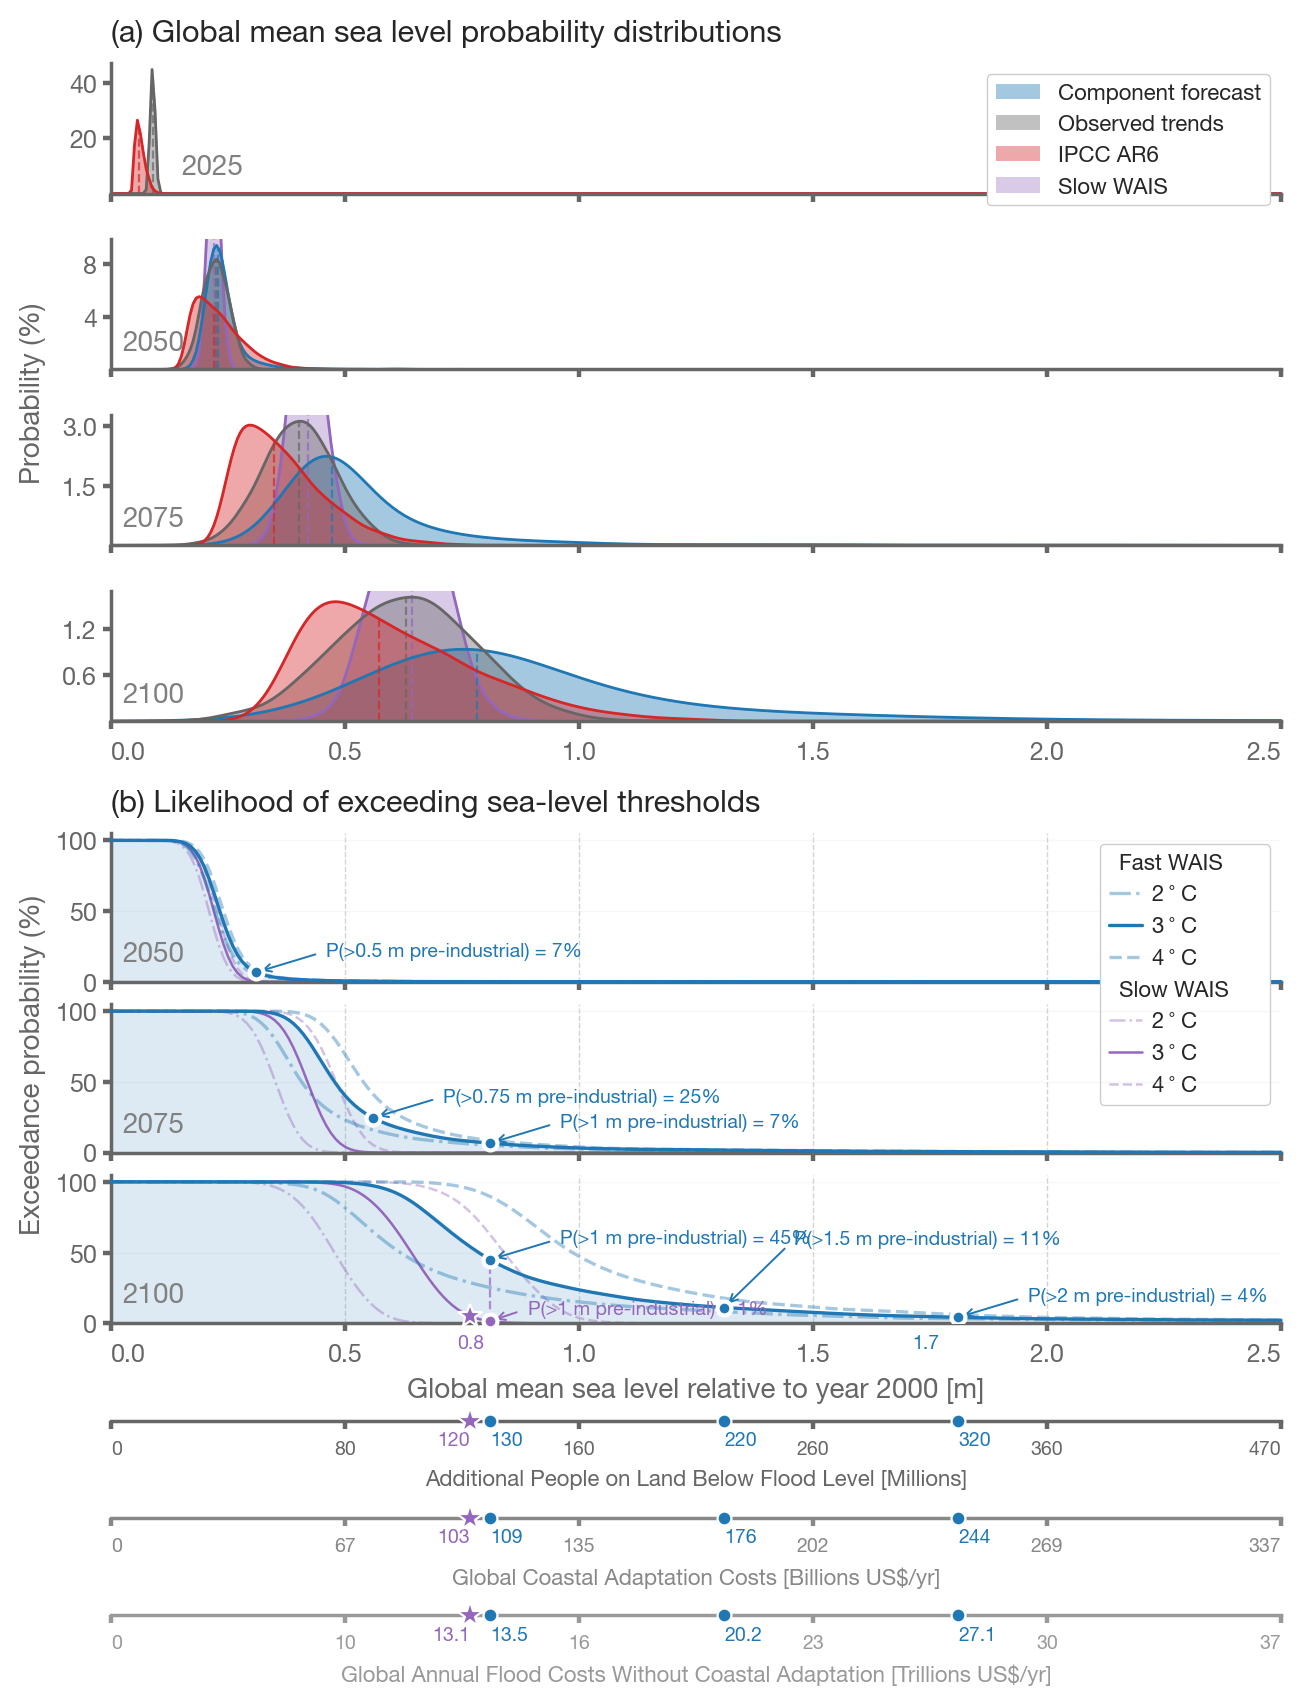
\includegraphics[width=0.85\textwidth]{fig2v2_ridge_exceedance.png}
\caption{\textbf{Global mean sea-level probabilities.}
(a) Probability distributions for different forecasting approaches and the IPCC projections. The `slow WAIS' scenario (purple, clipped for clarity) assumes sustained mass loss at approximately modern rates (Scenario 1). Vertical dashed lines indicate the respective medians. 
(b) Probability of exceeding a given sea-level threshold for different warming trajectories including the WAIS scenario mixture model that allows for fast mass loss (blue) and the slow WAIS scenario (purple). Lower axes show estimates of the corresponding number of people currently living on land that will be below flood level \citep{Kulp2019} and financial costs \citep{Tiggeloven2020,Jevrejeva2018} (Supplementary Material). Stars indicate the 5\% exceedance probability.}
\label{fig:ridge_projections}
\end{figure}

Relative to pre-industrial GMSL (adding $\sim$0.19 m of observed rise through 2000), these forecasts correspond to medians of 0.98--1.35 m of global mean sea level rise across the policy-relevant pathways. The probability of exceeding 1 m relative to pre-industrial by 2100 is 47\% under 2 $^\circ$C warming, 76\% under 3 $^\circ$C, and 96\% under 4 $^\circ$C warming trajectory. The probability of exceeding 2 m relative to pre-industrial by 2100 is approximately 10\%, with a minimum of 6\% if warming is held below 2 $^\circ$C. Under the condition that WAIS loses ice slowly, the probability of exceeding 1 m of sea level rise relative to pre-industrial levels drops to zero for less than 3 $^\circ$C of warming, implying lower flood risks for tens of millions of people and reduced costs of adaptation and damages of order trillions of US dollars (Fig. \ref{fig:ridge_projections}b). 

Our forecasts suggest that WAIS is likely to become the dominant source of sea-level rise before the end of the century (Fig. \ref{fig:components_voi}a). When that happens is uncertain and depends on how quickly emissions decrease. The stack of mean values shows the relative contributions of the primary sea-level contributors, which that the thermosteric component likely will remain the single largest contributor unless WAIS mass losses over take it. Greenland and mountain glaciers will continue to lose mass and contribute to sea level rise throughout the 21st century. 

The distribution of the uncertainties shows a clear separation between the predictable and, currently unpredictable components (Fig. \ref{fig:components_voi}b). These results show that WAIS accounts for virtually all of the variance, and approximately 92\% of the confidence interval, in future sea-level rise. The other sea level contributors, all of which have calibrated sensitivities to global mean surface temperature, contribute approximately 1\% to the total variance and 8\% to the 90\% (CI) uncertainty range across the plausible warming scenarios. As a result, the within-scenario 90\% uncertainty range (1.47 m for 3 $^\circ$C) is four times larger than the spread across warming scenario medians (0.37 m from 2--4 $^\circ$C). This picture is fundamentally different under the condition that WAIS loses mass slowly. In the slow-WAIS scenario, the warming-sensitive components become the largest contributors to the uncertainty (righthand column of Fig. \ref{fig:components_voi}b). The relative magnitude of uncertainties reveals that sea-level risk decomposes into two approximately orthogonal dimensions, each addressed by a distinct class of societal response.

\subsection*{Orthogonal dimensions of sea-level risk}

The first risk dimension is sensitive to emissions reduction. The temperature-dependent components are sensitive to changes in global mean surface temperature. In this work, we calibrate the sensitivities using decades of observations. Their collective contribution shifts systematically across warming trajectories and is reducible by emissions cuts (Fig. \ref{fig:components_voi}a). Under the `slow WAIS' scenario, the forecast narrows to a 90\% range of only $\sim$14 cm, an order of magnitude narrower than the full scenario cast that allows for rapid mass loss from WAIS due to internal feedbacks (Fig.~\ref{fig:ridge_projections}). In the slow scenario, emissions policy is the primary lever for managing risk: the difference between 2$\,^\circ$C and 4$\,^\circ$C warming is roughly 20 cm of additional rise, which roughly translates to 30 million additional people exposed to coastal flood risks and US\$50B/yr in coastal adaptation costs.

The second risk dimension is relatively insensitive to emissions reductions. WAIS dynamics accounts for virtually all of the total forecast variance and is largely decoupled from the emission pathway. The tail of the forecast distribution---the outcomes that drive the most severe human and economic consequences---is controlled almost entirely by whether WAIS retreat remains gradual at modern rates of loss or transitions to rapid, irreversible retreat. Emissions reduction decreases the median but does not substantively change the tail of the distribution. The probability of exceeding 2 m relative to pre-industrial is 6\% under the 2$\,^\circ$C trajectory and 14\% under 4$\,^\circ$C, with a 10\% probability across emission scenarios. The 6\% lower bound on this range highlights the fact that emission reductions alone cannot retire the high risk outcomes.

%% ---- Figure 4: Component decomposition and VoI ----
\begin{figure}[t]
\centering
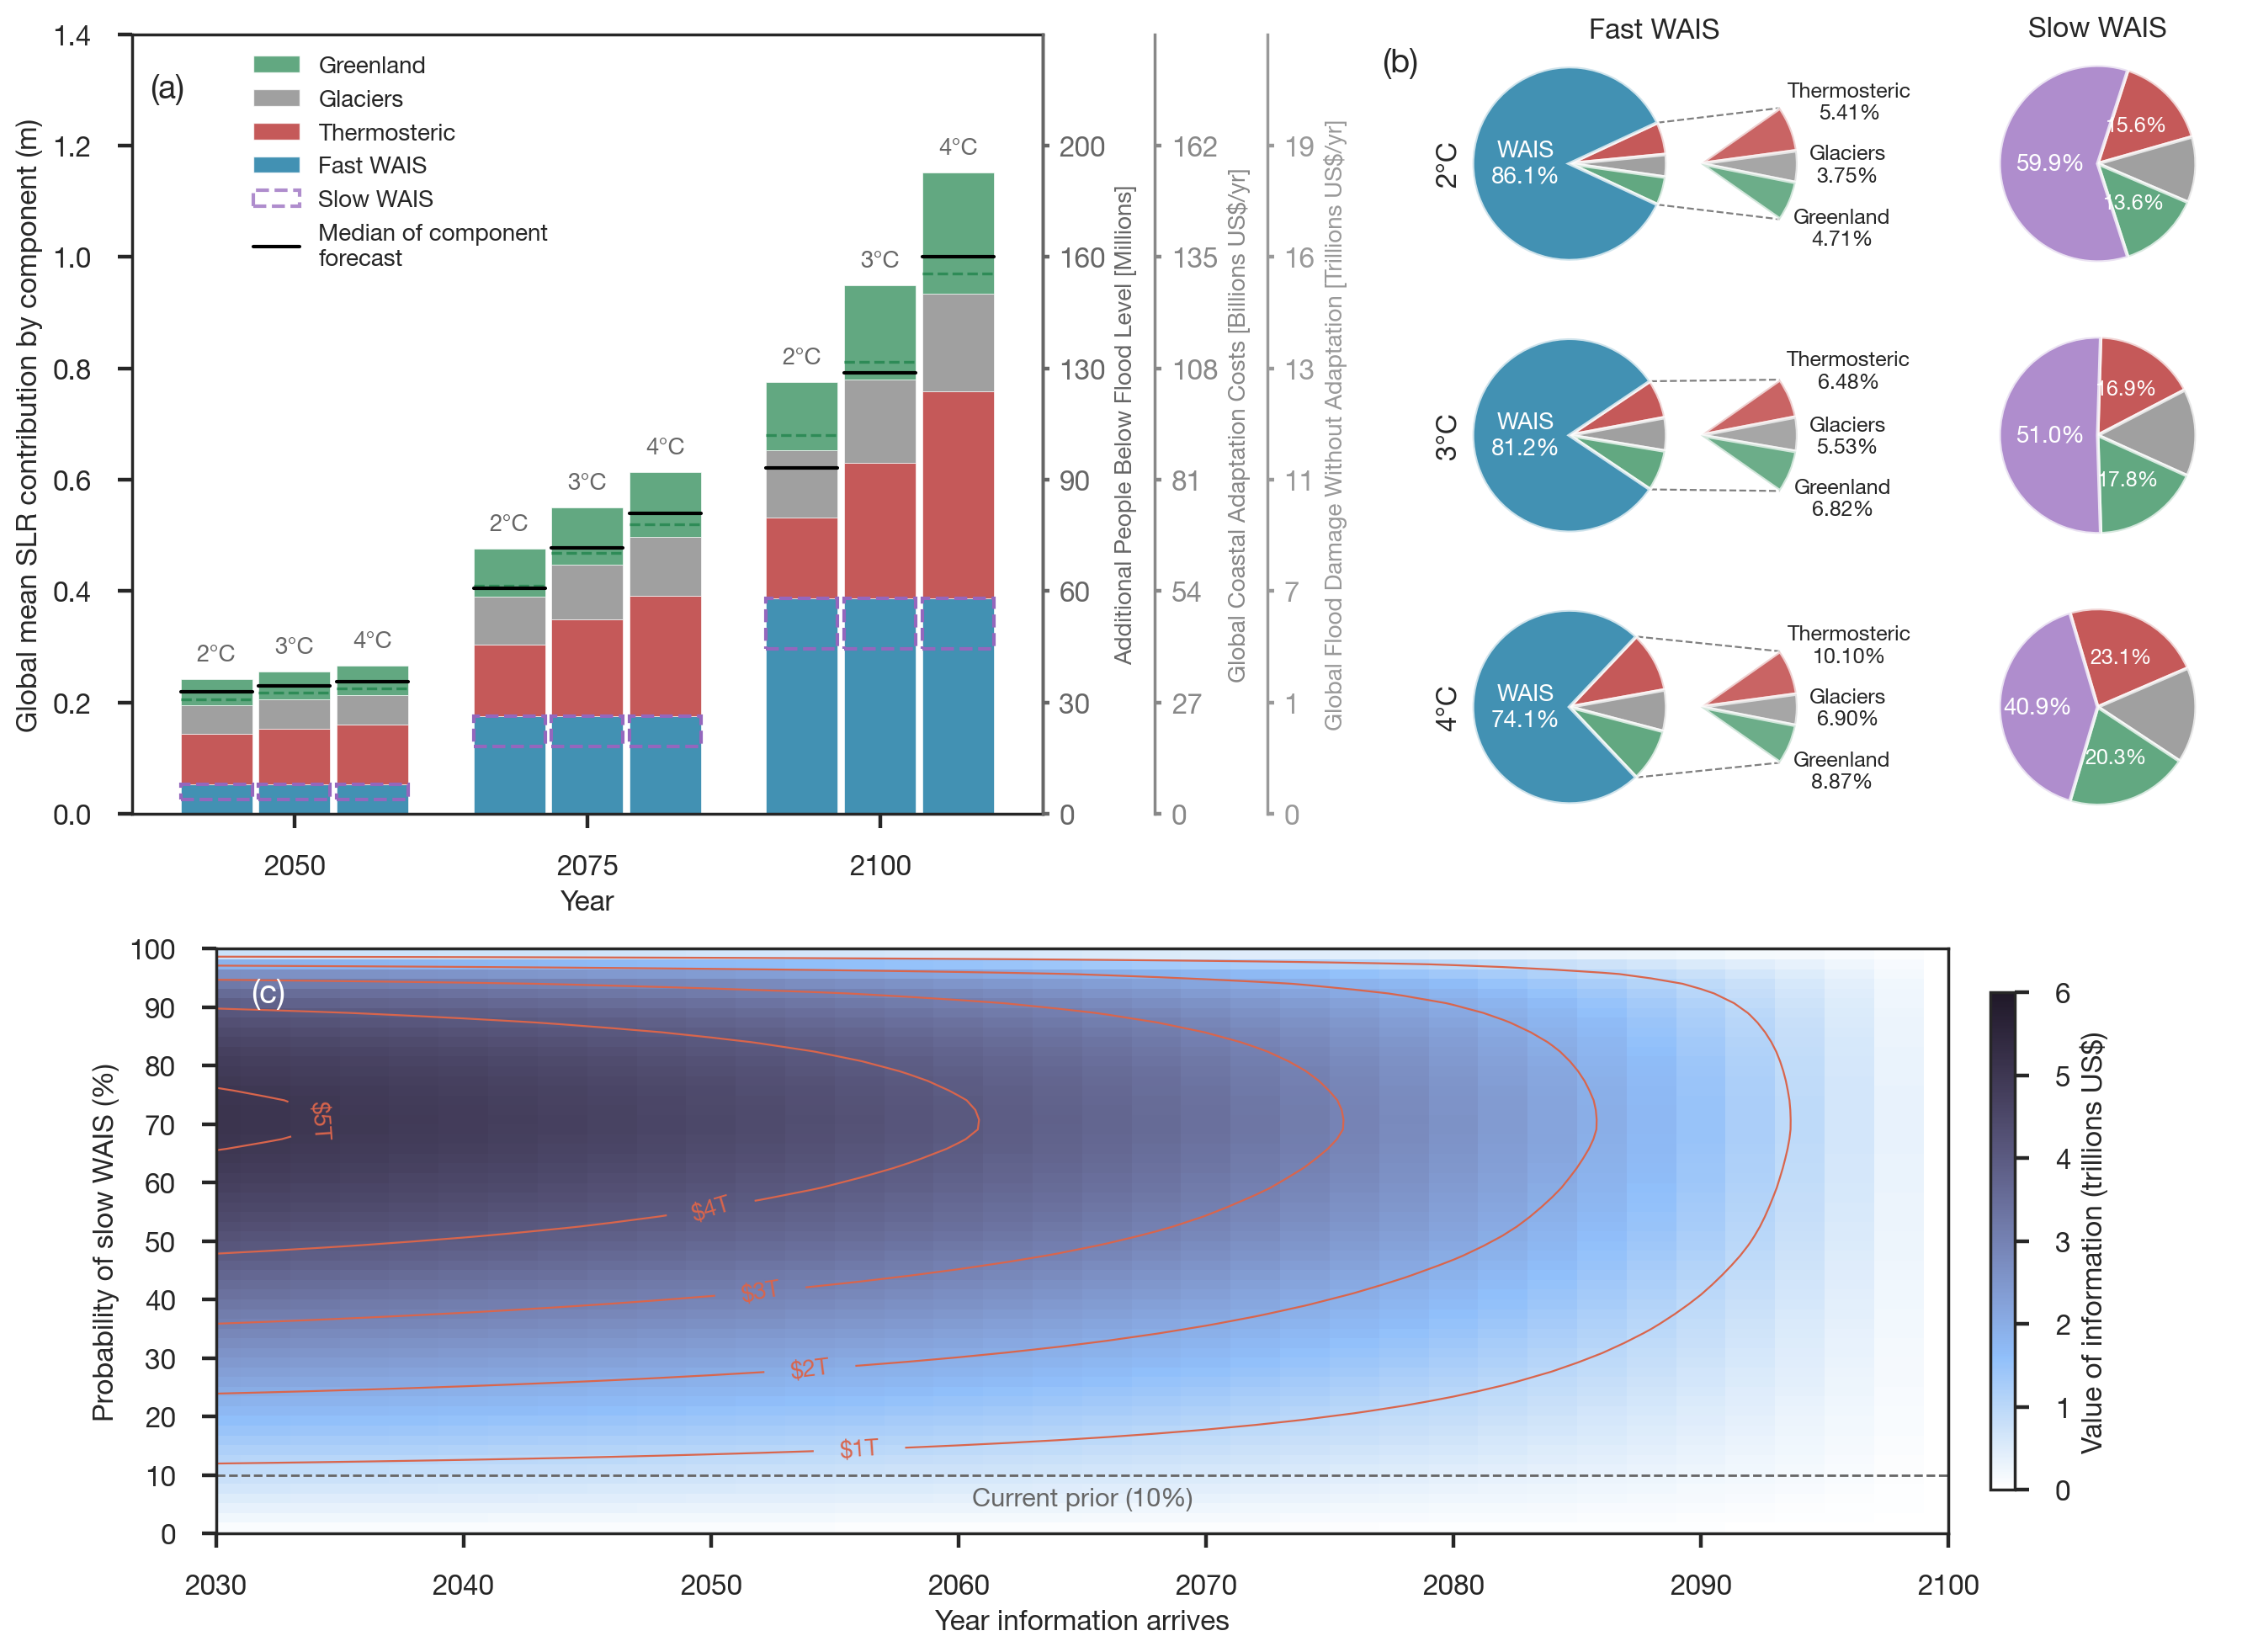
\includegraphics[width=\textwidth]{fig_slr_by_component_v2.png}
\caption{\textbf{Component contributions, variance decomposition, and value of information.}
\textbf{(a)} 21st century mean GMSLR contribution by component and respective societal costs. Green dashed lines within Greenland bars partition discharge anomaly (below) from SMB anomaly (above). The purple box shows how much WAIS will contribute if it loses mass slowly while the rest of the blue bar shows the potential SLR from rapid ice loss. 
\textbf{(b)} Variance-fractions at 2100. WAIS accounts for 97--99\% of total forecast variance when rapid ice loss is possible. Fan breakouts show the non-WAIS contributions. If WAIS loses moss slowly, the variance distributions fundamentally shift (right column) 
\textbf{(c)} Financial value of resolving WAIS uncertainty as a function of when information arrives. Contours and colormap in trillions US\$ based on coastal adaptation costs (Supplemental Material). The plot shows that information has more value if it arrives early enough to inform key decisions and if it provides sufficient confidence that WAIS will lose mass slowly, allowing planning around lower future sea levels.}
\label{fig:components_voi}
\end{figure}

The risks and costs to coastal communities helps to highlight the dichotomy between the two possible scenarios of fast vs slow WAIS mass loss, or equivalently, emissions-insensitive vs emissions sensitive (Figs. \ref{fig:ridge_projections} and \ref{fig:components_voi}a). The difference at the 5\% exceedance probability, one possible design threshold for coastal adaptation that we denote by stars in Fig. \ref{fig:ridge_projections}b, is 1.4 m of sea-level rise by 2100 under the current policy warming trajectory (3 $^\circ$C). This difference translates into roughly 260M more people exposed to annual flood risks, US$182B/yr in coastal adaptation, and US$18.2T/yr ($\sim$16\% global GDP per year) in coastal flood damages without further adaptation. These large numbers reflect global population densities, with the highest densities near coastlines, and the fact that the locations of coastal communities and infrastructure are calibrated to lower sea levels. For intuition, the fast-WAIS scenario at 5\% exceedance implies an order of magnitude more sea level rise in the next 75 years than was experienced in the past 125 years, while the slow-WAIS scenario implies a factor of 3.5 more rise.

These costs show that resolving the question of WAIS mass loss rates is one of the most valuable actions modern science in terms of savings in lives and financial costs, to say nothing of coastal ecosystems (\ref{fig:components_voi}c). A simple value-of-information estimate shows a peak value $>$US\$5T for a high degree of certainty in a slow-WAIS future, so long as that information arrives in time to support key decisions. The time pressure combined with the short data record and complexity of the ice sheet make this a challenging goal to meet on its own. The current level of funding, which is of order tens of millions per year globally \citep{Catania2022}, can be best described as unserious against these risks and challenges. From a purely financial perspective and when measured against the costs of uncalibrated coastal development and damages, research aimed at resolving the question of how fast will WAIS lose mass is justified at the US\$1B/yr or more. 

Scientific research is a necessary condition for providing actionable information for coastal adaptation, but it is as likely as not that further research will add to the growing evidence to support rapid WAIS mass loss rather than build confidence in a slow-WAIS future \citep{Fricker2025}. Because the probability of $>2$ m by 2100 is non-negligible, a lack of evidence for sea-level rise $\sim$ 1 m will force major decisions on coastal planning, adaptation, and managed retreat of people from coastlines to be made under large uncertainties. The extent of these uncertainties and scale of cost in terms of lives, property, and ecosystems forces the question: Can we take action to increase the potential stability of West Antarctica? Recently, some research directions have been proposed to answer this question \citep{MacAyeal2024} and as with any nascent research, there are many unresolved concerns about the feasibility, unintended consequences, and governance of these interventions \citep{ 

%\subsection*{Broader implications}

%The data-driven framework presented here is not a replacement for process models, which remain essential for understanding the mechanisms of ice-sheet change. Our framework is complementary: an independent, data-driven estimate that makes its assumptions and limitations explicit, provides an observational benchmark against which process models can be tested, and produces conditional distributions that reflect what the data currently support. We consider robust, well-calibrated process models to be high-value targets for research and development, but the evidence suggests these models are not ready to be used for planning that costs billions of dollars and impacts millions of lives.

%We emphasize that the disconnect between the high costs of sea-level rise and the large uncertainties in current sea-level projections is a consequence of chronic under-investment compounded by the lack of institutional homes able to focus on translating knowledge gained through basic scientific research into forecasts for coastal communities in the way that, for example, the National Weather Service has traditionally done \citep{Catania2022}. A specific example is that modeling efforts for ISMIP6, which informed IPCC AR6 projections, were largely unfunded, leading to a dearth of model runs and near-absence of model parameter-sensitivity studies \citep{Aschwanden2021}. The world is going to endure high costs from sea-level rise (Fig. \ref{fig:ridge_projections}b). The questions are: how high will those costs be, and will we invest now to understand where and how to target funding to reduce the harm to people, ecosystems, and infrastructure, or continue on our current path? Our analysis shows that this investment must be directed along two independent axes---reducing emissions to compress the predictable components, and understanding and potentially stabilizing the West Antarctic Ice Sheet to address the dominant, emission-insensitive uncertainty that defines the upper bound of 21st-century sea-level rise.


%% ================================================================
%% REFERENCES
%% ================================================================

\bibliographystyle{sciencemag}
\bibliography{references}

\end{document}     